% ============================================================================
% CHAPTER 6 — ESLM-AE: EXTENDED SLM WITH AUTOENCODER FOR DCO-OFDM
% ============================================================================
\chapter{ESLM-AE: Extended SLM with Autoencoder for DCO-OFDM}
\label{ch:eslm_ae}

\begin{motivation}
    The GA-SLM of the previous chapter stays within the SLM framework but
    uses an expensive online search.  Can we instead \emph{learn} the optimal
    phase factors \emph{once} during offline training, then apply them
    instantly at transmission time?
    Hao et al.\ (2019) proposed the \textbf{Extended SLM combined with
    Autoencoder (ESLM-AE)} scheme for DCO-OFDM systems used in Visible
    Light Communications (VLC).  The key innovation is to extend the SLM
    phase alphabet from a discrete set to the \emph{full continuous range}
    $[0, 2\pi)$, and use an autoencoder to learn the optimal phase factors
    via backpropagation~\cite{hao2019extended}.
\end{motivation}


% ----------------------------------------------------------------------------
\section{Conceptual Overview}
\label{sec:eslm_concept}
% ----------------------------------------------------------------------------

\subsection{DCO-OFDM: A Quick Primer}

ESLM-AE targets \textbf{DC-biased Optical OFDM (DCO-OFDM)}, a modulation
scheme used in optical wireless communications (VLC, Li-Fi).
In DCO-OFDM, the electrical OFDM signal must be real-valued and non-negative
(since light intensity cannot be negative).  This is achieved
by~\cite{hao2019extended}:
\begin{enumerate}
    \item \textbf{Hermitian symmetry:} enforcing conjugate symmetry on the
          frequency-domain data so the IFFT output is real:
          $X_{N-k} = X_k^*$ for $k = 1, \dots, N/2-1$.
    \item \textbf{DC bias:} adding a positive DC offset to shift the entire
          signal above zero.
\end{enumerate}

DCO-OFDM suffers from even higher PAPR than RF OFDM because the Hermitian
symmetry constraint reduces the degrees of freedom, and the DC bias further
increases peak power~\cite{hao2019extended}.

\subsection{The ``Extended'' in ESLM}

Classical SLM restricts phase factors to a finite alphabet
(e.g., $\{+1, -1, +j, -j\}$).
The \textbf{Extended SLM (ESLM)} removes this restriction:
phase factors can take \emph{any} value on the unit
circle~\cite{hao2019extended}:
\begin{equation}
    \psi_k \in \{e^{j\varphi_k} : \varphi_k \in [0, 2\pi)\}.
    \label{eq:eslm_continuous_phase}
\end{equation}

This vastly increases the search space, making exhaustive search
impossible.  The autoencoder is the mechanism that navigates this
expanded space efficiently~\cite{hao2019extended}.


% ----------------------------------------------------------------------------
\section{System Model and Architecture}
\label{sec:eslm_architecture}
% ----------------------------------------------------------------------------

\begin{figure}[H]
    \centering
    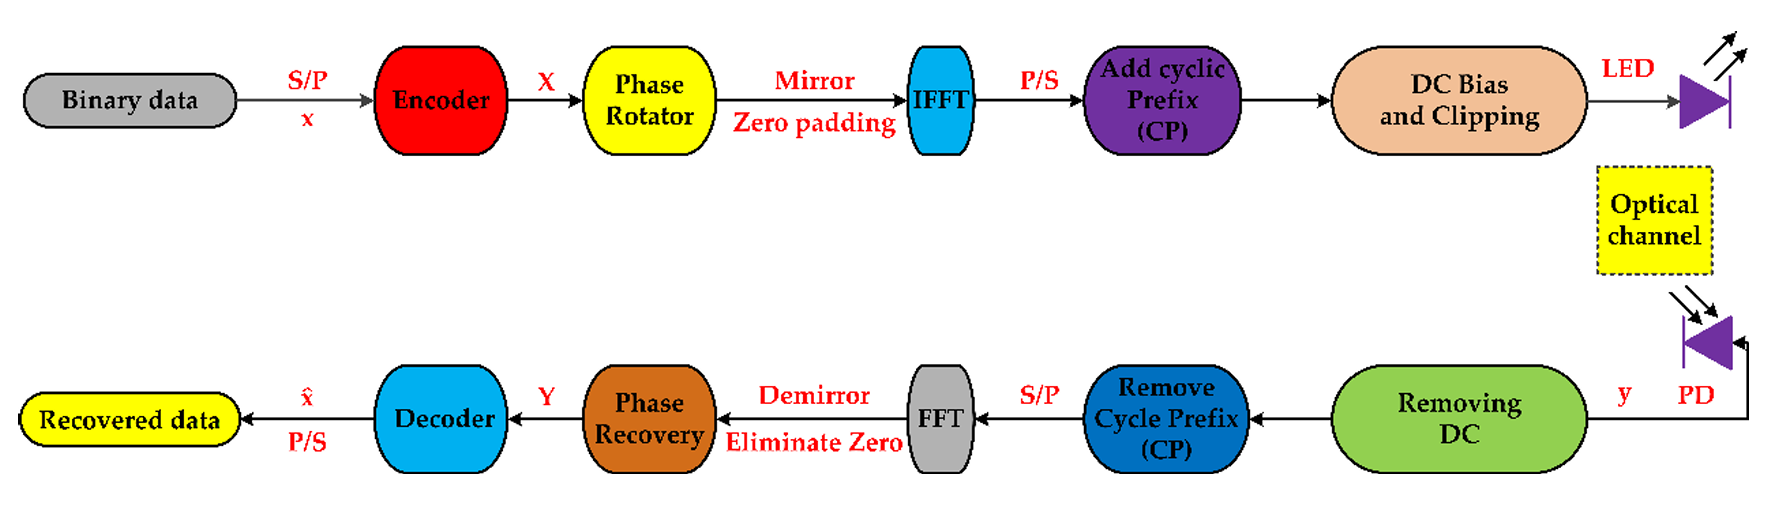
\includegraphics[width=0.95\linewidth]{Figures/29_eslm_ae_overview.png}
    \caption{Overall system model of the ESLM-AE scheme for DCO-OFDM.
             The autoencoder learns to generate optimal phase rotation
             factors that minimize PAPR while preserving signal recoverability.
             Reproduced from~\cite{hao2019extended}.}
    \label{fig:eslm_overview}
\end{figure}

\subsection{Encoder (Transmitter)}

The encoder consists of two stages~\cite{hao2019extended}:

\paragraph{Stage 1: Phase Factor Generation.}
A neural network takes the frequency-domain data $\bm{X}$ as input and
produces $N$ phase factors:
\begin{equation}
    \bm{\varphi} = \mathcal{N}_{\mathrm{enc}}\!\bigl(\bm{X};\;\bm{\theta}\bigr),
    \qquad \varphi_k \in [0, 2\pi).
    \label{eq:eslm_phase_gen}
\end{equation}

\paragraph{Stage 2: SLM Phase Rotation + IFFT.}
The generated phases are applied to the data (exactly as in classical SLM),
followed by the IFFT~\cite{hao2019extended}:
\begin{equation}
    \bm{x}_{\mathrm{SLM}} = \mathrm{IFFT}\!\bigl\{\bm{X} \odot
    [e^{j\varphi_0}, e^{j\varphi_1}, \dots, e^{j\varphi_{N-1}}]^T\bigr\}.
    \label{eq:eslm_rotation}
\end{equation}

\begin{figure}[H]
    \centering
    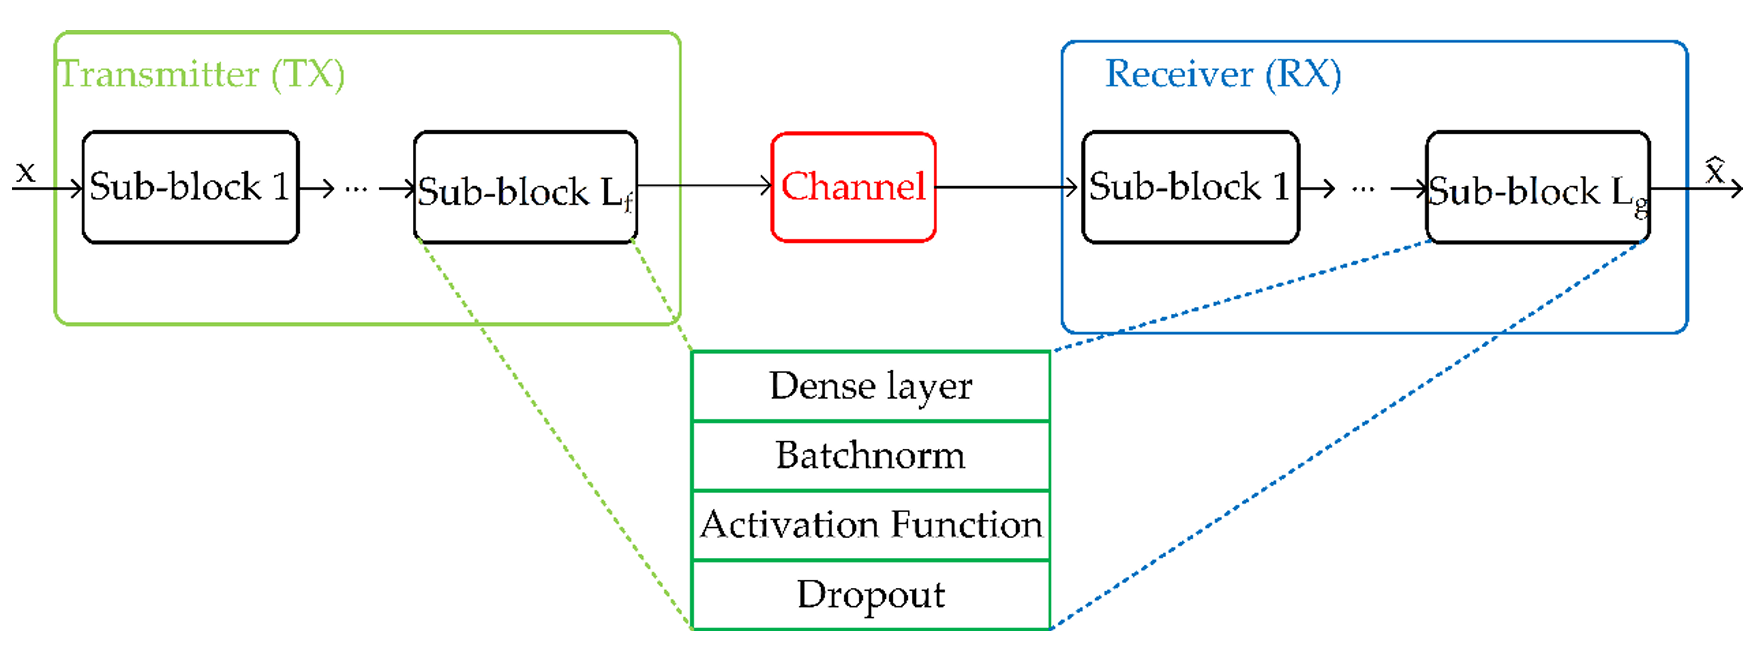
\includegraphics[width=0.90\linewidth]{Figures/30_eslm_ae_autoencoder.png}
    \caption{Autoencoder structure used in ESLM-AE.
             The encoder generates continuous-valued phase rotation factors,
             and the decoder recovers the original data after
             the DCO-OFDM channel.
             Reproduced from~\cite{hao2019extended}.}
    \label{fig:eslm_autoencoder}
\end{figure}

\begin{figure}[H]
    \centering
    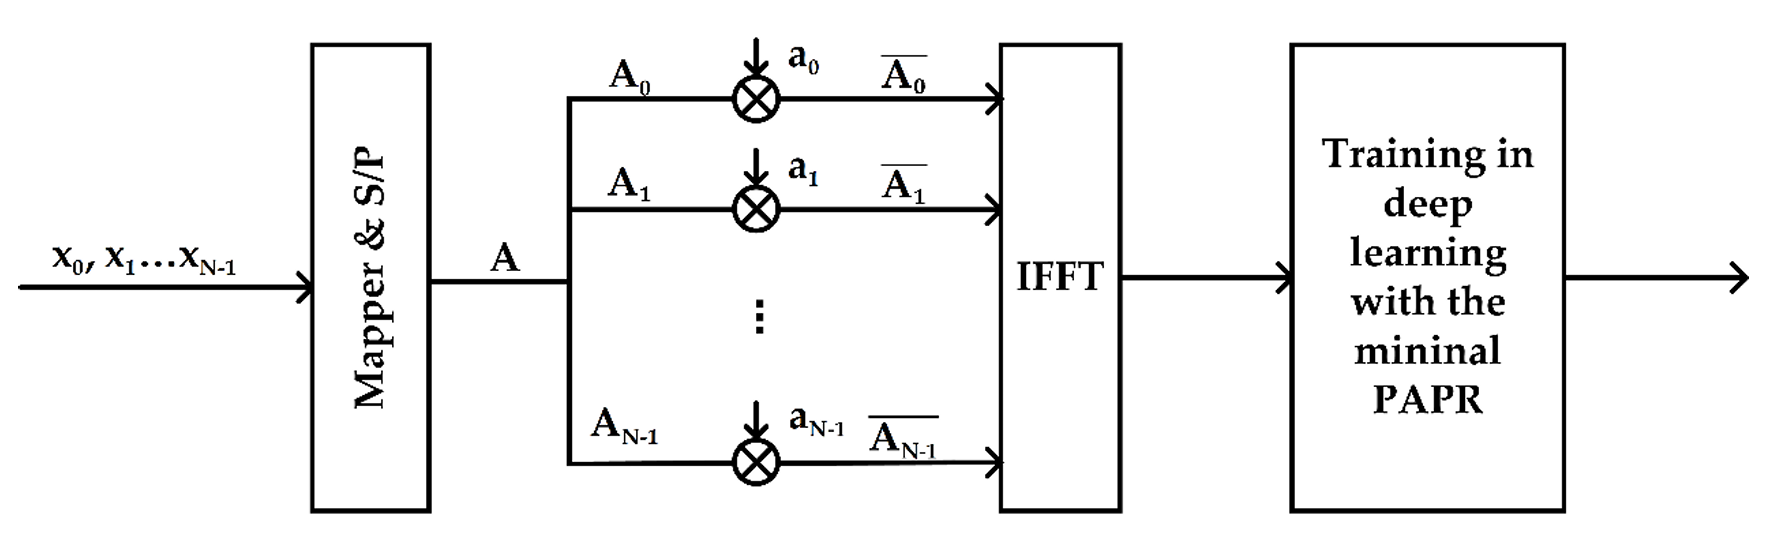
\includegraphics[width=0.80\linewidth]{Figures/31_eslm_ae_phase_rotator.png}
    \caption{Phase rotation operation in the ESLM transmitter.
             Each frequency-domain symbol $X_k$ is multiplied by a learned
             phase factor $e^{j\varphi_k}$ before the IFFT.  The phase
             factors are generated by the neural network encoder.
             Reproduced from~\cite{hao2019extended}.}
    \label{fig:eslm_rotator}
\end{figure}

\begin{keyinsight}
    Unlike PRNet, the ESLM-AE encoder does \emph{not} replace the IFFT
    or produce an arbitrary nonlinear transformation.  It generates
    \emph{phase factors} that are applied within the standard SLM
    framework.  This means the transmitted signal is still a valid OFDM
    signal with a known structure---only the phase factors are
    learned~\cite{hao2019extended}.
\end{keyinsight}

\subsection{Decoder (Receiver)}

The decoder receives the signal after the optical channel (which includes
LED nonlinearity, optical noise, and multipath effects in VLC) and
reconstructs the original data.  It learns to implicitly determine
which phase factors were used and reverse the rotation---eliminating
the need for explicit side information~\cite{hao2019extended}.


% ----------------------------------------------------------------------------
\section{Training Procedure}
\label{sec:eslm_training}
% ----------------------------------------------------------------------------

The ESLM-AE is trained end-to-end with a loss function that combines
PAPR reduction and reconstruction accuracy~\cite{hao2019extended}:
\begin{equation}
    \mathcal{L}_{\mathrm{ESLM}}
    = \beta \cdot \mathcal{L}_{\mathrm{PAPR}}
    + (1 - \beta) \cdot \mathcal{L}_{\mathrm{MSE}},
    \label{eq:eslm_loss}
\end{equation}
where $\beta$ is the balancing parameter.

A critical subtlety: the IFFT operation in \eqref{eq:eslm_rotation} is
a linear operation and is therefore \textbf{differentiable}---gradients
can flow through it from the PAPR loss back to the phase-generation
network.  This allows the phase factors $\bm{\varphi}$ to be optimized
directly by backpropagation~\cite{hao2019extended}.


% ----------------------------------------------------------------------------
\section{Simulation and System Parameters}
\label{sec:eslm_params}
% ----------------------------------------------------------------------------

\begin{table}[H]
    \centering
    \caption{Simulation parameters for ESLM-AE~\cite{hao2019extended}.}
    \label{tab:eslm_params}
    \begin{tabular}{@{} l l @{}}
        \toprule
        \textbf{Parameter} & \textbf{Value} \\
        \midrule
        Number of subcarriers ($N$) & 128 \\
        Modulation scheme & 4-QAM (QPSK) \\
        OFDM type & DCO-OFDM \\
        Hermitian symmetry & Enforced \\
        DC bias & $7$~dB \\
        Channel models & LOS, Rician, Diffuse \\
        SLM candidates ($U$) & 4, 8, 16 \\
        Phase alphabet (classical SLM) & $\{+1, -1\}$ \\
        Phase range (ESLM) & $[0, 2\pi)$ continuous \\
        Hidden layers & 3 \\
        Neurons per layer & 256 \\
        Training epochs & 300 \\
        Learning rate & $10^{-3}$ \\
        Optimizer & SGD with Adam \\
        \bottomrule
    \end{tabular}
\end{table}


% ----------------------------------------------------------------------------
\section{Results and Analysis}
\label{sec:eslm_results}
% ----------------------------------------------------------------------------

\subsection{PAPR Reduction}

\begin{figure}[H]
    \centering
    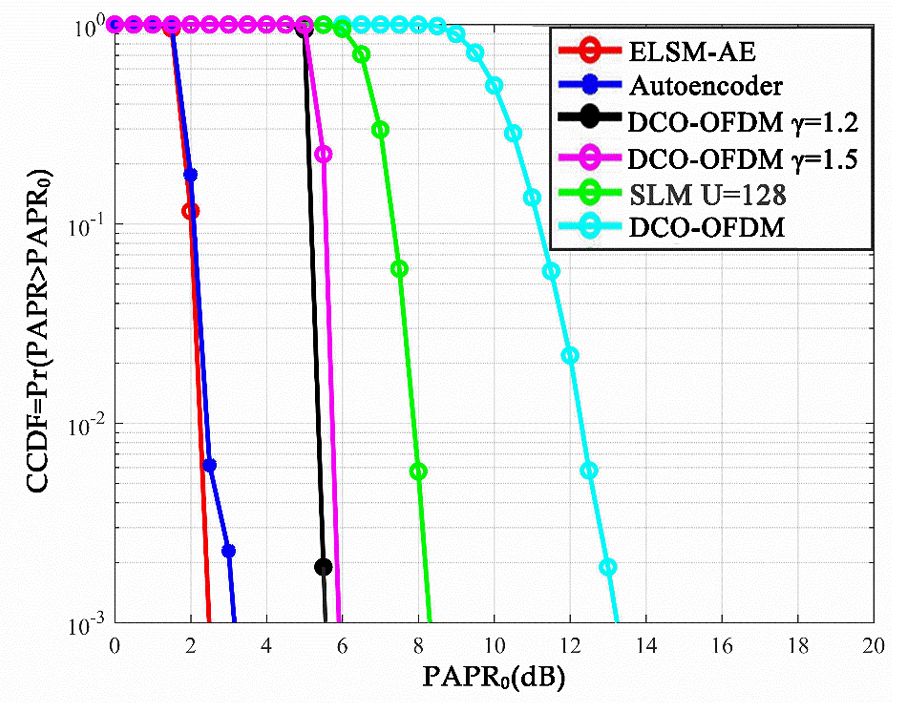
\includegraphics[width=0.70\linewidth]{Figures/32_eslm_ae_ccdf.png}
    \caption{CCDF of PAPR for ESLM-AE compared to conventional SLM
             and the original DCO-OFDM signal ($N=128$).
             The autoencoder-optimized continuous phase factors
             outperform discrete-alphabet SLM.
             Reproduced from~\cite{hao2019extended}.}
    \label{fig:eslm_ccdf}
\end{figure}

\begin{keyinsight}
    ESLM-AE achieves PAPR reduction comparable to or exceeding
    conventional SLM with $U=16$ discrete candidates, while using
    only a \emph{single} forward pass through the encoder network.
    The continuous phase alphabet provides additional freedom that
    discrete-alphabet SLM cannot exploit~\cite{hao2019extended}.
\end{keyinsight}

\subsection{BER Performance Under Different Channels}

A major contribution of this paper is evaluating BER under realistic
VLC channel conditions~\cite{hao2019extended}:

\begin{figure}[H]
    \centering
    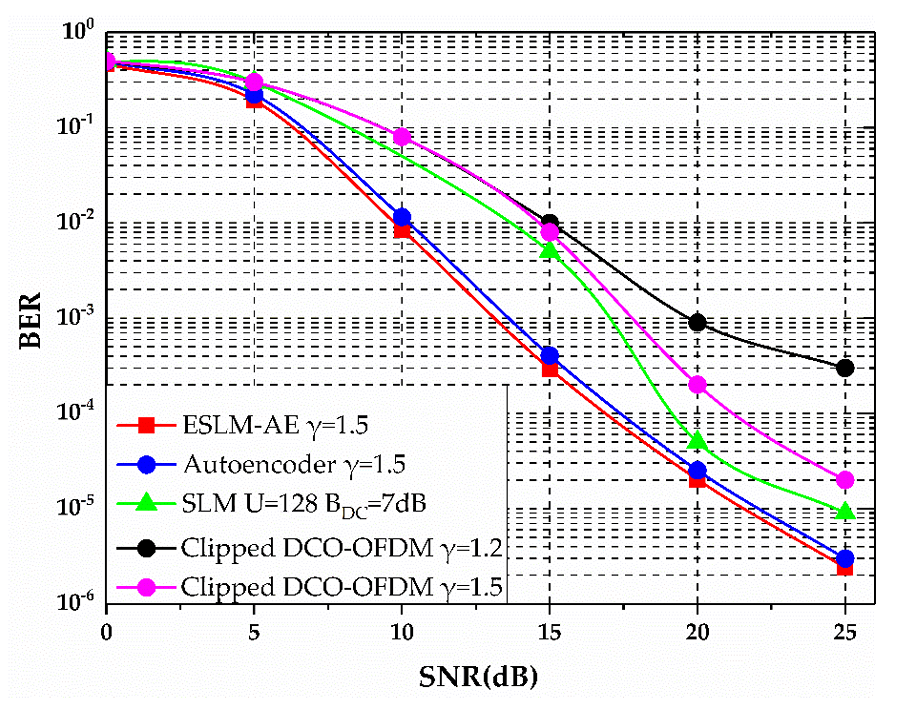
\includegraphics[width=0.70\linewidth]{Figures/33_eslm_ae_ber_los.png}
    \caption{BER vs.\ SNR for ESLM-AE under Line-of-Sight (LOS) channel.
             ESLM-AE maintains good BER performance comparable to
             conventional SLM.
             Reproduced from~\cite{hao2019extended}.}
    \label{fig:eslm_ber_los}
\end{figure}

\begin{figure}[H]
    \centering
    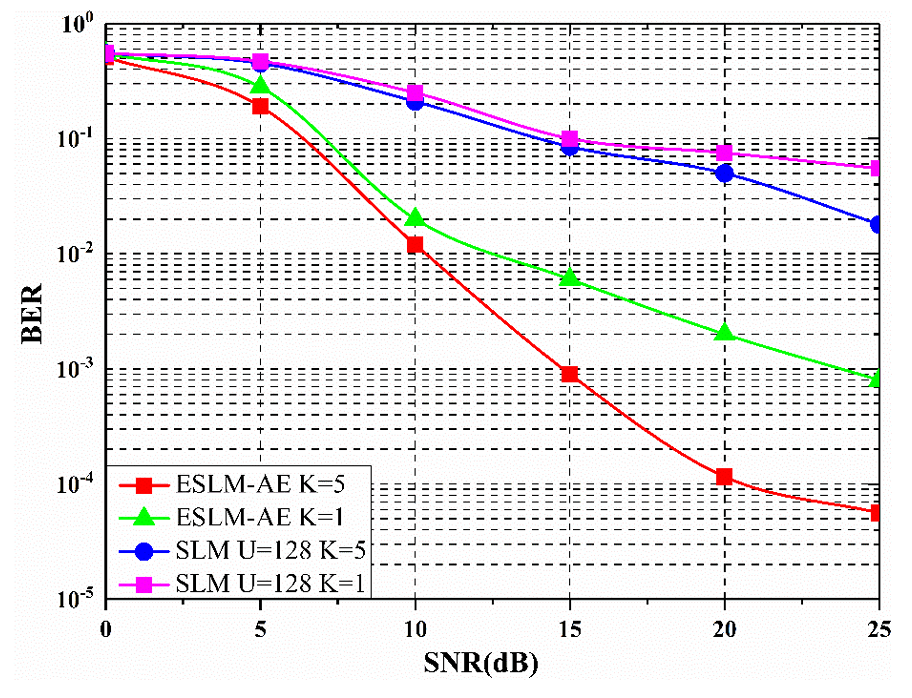
\includegraphics[width=0.70\linewidth]{Figures/34_eslm_ae_ber_rician.png}
    \caption{BER vs.\ SNR for ESLM-AE under Rician fading channel.
             Performance degrades slightly compared to LOS but
             remains competitive.
             Reproduced from~\cite{hao2019extended}.}
    \label{fig:eslm_ber_rician}
\end{figure}

\begin{figure}[H]
    \centering
    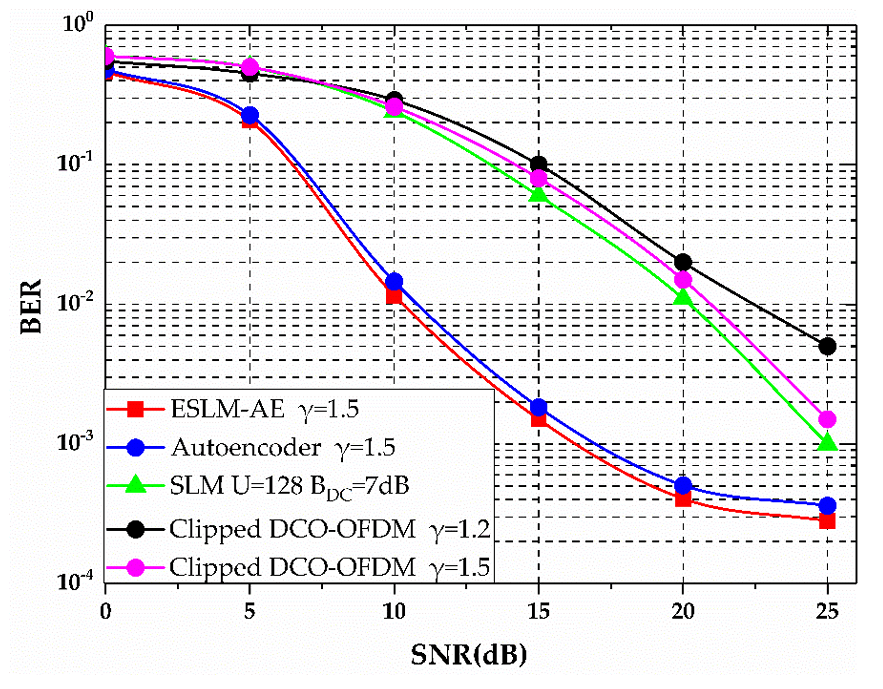
\includegraphics[width=0.70\linewidth]{Figures/35_eslm_ae_ber_dow.png}
    \caption{BER vs.\ SNR for ESLM-AE under diffuse optical wireless (DOW)
             channel.  The multipath-rich environment poses a harder challenge.
             Reproduced from~\cite{hao2019extended}.}
    \label{fig:eslm_ber_dow}
\end{figure}

\begin{figure}[H]
    \centering
    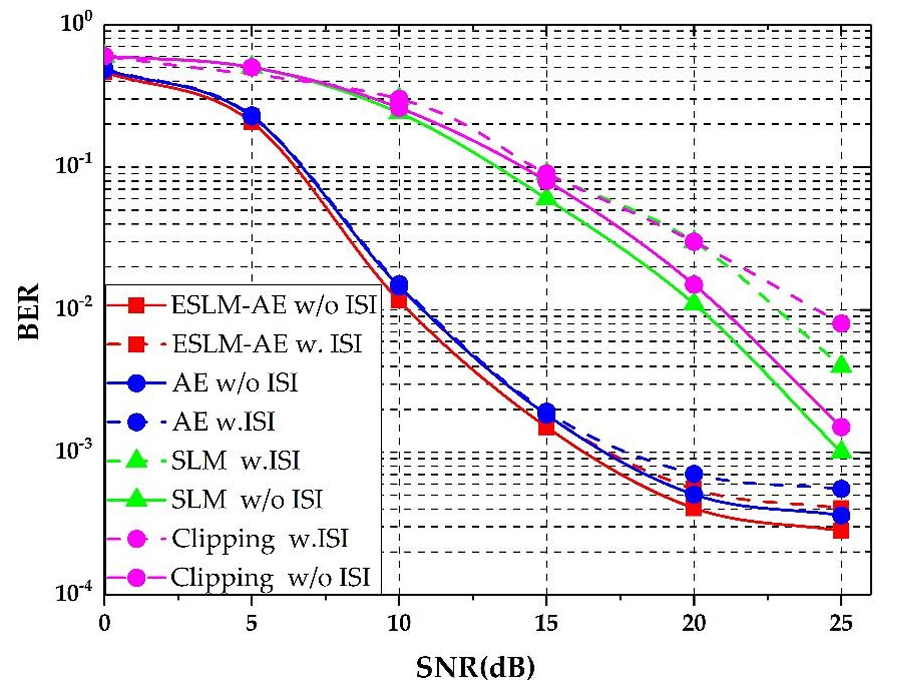
\includegraphics[width=0.70\linewidth]{Figures/36_eslm_ae_ber_isi.png}
    \caption{BER vs.\ SNR for ESLM-AE under DOW channel with and without
             Inter-Symbol Interference (ISI) by using a shorter CP.
             ESLM-AE exhibits robustness against ISI.
             Reproduced from~\cite{hao2019extended}.}
    \label{fig:eslm_ber_isi}
\end{figure}


% ----------------------------------------------------------------------------
\section{Common Misconceptions}
\label{sec:eslm_misconceptions}
% ----------------------------------------------------------------------------

\begin{misconception}
    \textbf{``ESLM-AE is the same as PRNet applied to optical OFDM.''} \\
    No.  The key architectural difference is that ESLM-AE generates
    \emph{phase factors} within the standard SLM framework and uses the
    standard IFFT.  PRNet replaces the IFFT entirely with a learned
    nonlinear mapping.  ESLM-AE preserves the OFDM signal structure;
    PRNet does not~\cite{hao2019extended,kim2017novel}.
\end{misconception}


% ----------------------------------------------------------------------------
\section{Limitations and Open Problems}
\label{sec:eslm_limitations}
% ----------------------------------------------------------------------------

\begin{enumerate}
    \item \textbf{DCO-OFDM specific:}
          The architecture and training assume DCO-OFDM with Hermitian
          symmetry.  Adapting to RF OFDM (complex-valued) requires
          modifications~\cite{hao2019extended}.

    \item \textbf{Moderate subcarrier count:}
          Evaluated with $N=128$.  Scalability to larger systems is not studied.

    \item \textbf{Limited channel modeling:}
          While three channel types are tested (a major improvement over
          Kim~2017), more complex VLC scenarios (e.g., multi-user, MIMO)
          are not addressed~\cite{hao2019extended}.

    \item \textbf{Phase factor generalization:}
          The learned phase factors may not generalize well to data
          distributions or channel conditions not seen during training.
\end{enumerate}


% ----------------------------------------------------------------------------
\section{Connection to Other Approaches}
\label{sec:eslm_connections}
% ----------------------------------------------------------------------------

ESLM-AE bridges the gap between classical SLM and deep learning:
\begin{itemize}
    \item From PRNet, it inherits the autoencoder training paradigm
          and joint loss function~\cite{kim2017novel}.
    \item From classical SLM, it preserves the phase-rotation structure,
          maintaining signal compatibility.
    \item The continuous phase extension anticipates the PR-DUN approach
          (next chapter), which also uses learned parameters within a
          structured algorithm~\cite{nguyen2022deep}.
\end{itemize}
